\documentclass[11pt]{article}
\title{MATH 222 Assignment 4}
\author{Sterling Laird - V00834995}
\date{February 25, 2019}

\usepackage{enumitem}
\usepackage{amsmath}
\usepackage{amssymb}
\usepackage{tikz}

\graphicspath{{./}}

\setlength{\parindent}{1.7cm}

\begin{document}

\maketitle
\pagebreak

\begin{enumerate}[]
\item
\item
Consider $n$ distinguishable elements and $n-2$ indistinguishable boxes. Count the number of ways to divide the elements into the boxes such that no box is empty for $n\geq 4$.\\
Clearly there are $S(n,n-2)$ such ways.\\
There are 2 possible cases for any such distribution as follows:
	\begin{enumerate}
	\item There are 3 elements that share a single box. There are $\binom{n}{3}$ ways to pick the 3 elements and since all other indistinguishable boxes must have only 1 element, there are $\binom{n}{3}$ ways total to arrange the elements in this case.
	\item There are 2 boxes which each contain 2 elements. There are $\binom{n}{4}$ ways to choose the elements and $\frac{\binom{4}{2}}{2} = 3$ ways to distribute the chosen elements into a box for a total of $3\binom{n}{4}$ ways to arrange the elements in this case.
	\end{enumerate}
This makes a total number of ways to distribute the elements of $\binom{n}{3}+3\binom{n}{4}$\\
$\therefore S(n,n-2)=\binom{n}{3}+3\binom{n}{4}$ for $n\geq 4$.
\item
We can use a generating function to get our result.\\
Consider the generating function in which the sum of coefficients of $x^i$ with $i\leq 35$ is our result:
	\begin{align}
		g(x)&=(x^0+x^1+x^2...)^6 \nonumber\\
		&=\frac{1}{(1-x)^6} \nonumber\\
	\end{align}
If we multiply $g(x)$ by $\frac{1}{1-x}=1+x+x^2+...$, the coefficient of $x^{35}$ is our result since the new $g(x)$ has coefficients which are cumulative of the old $g(x)$ coefficients. So:
	\begin{align}
		g(x)&=\frac{1}{(1-x)^6}\cdot \frac{1}{1-x} \nonumber\\
		&=\frac{1}{(1-x)^7} \nonumber\\
		&=\sum_{i=0}^{\infty} \binom{i+7-1}{7-1}x^i  \nonumber\\
		&=\sum_{i=0}^{\infty} \binom{i+6}{6}x^i \nonumber\\
	\end{align}
Clearly then, the coefficient of $x^{35}$, the number is of integers between 0 and 999999 with digits that sum to no more than 35, is $\binom{41}{6} = 4496388$
\item
Consider a hexagonal shaped room with the 6 walls labeled 0,1,2,3,4,5 in order around the room.\\
Let $c_i$ be the condition that the walls $i$ and $i+1\mod 5$ are the same color for $0\leq i\leq5$.\\
$N=10^6$\\
$N(c_i)=10^5$\\
$N({c_i}{c_j})=10^4$\\
$N({c_i}{c_j}{c_k})=10^3$\\
$N({c_i}{c_j}{c_k}{c_q})=10^2$\\
$N({c_i}{c_j}{c_k}{c_q}{c_r})=10$\\
$N({c_0}{c_1}{c_2}{c_3}{c_4}{c_5})=10$\\
$\overline{N} = 10^6 - \binom{6}{1}\cdot 10^5 + \binom{6}{2}\cdot 10^4 - \binom{6}{3}\cdot 10^3 + \binom{6}{4}\cdot 10^2 - \binom{6}{5}\cdot 10 + \binom{6}{6}\cdot 10$\\
$\overline{N} = 528450$
\item
	\begin{enumerate}[label=\alph*]
	\item For R to be an equivalence relation, it must be reflexive, symmetric, and transitive.\\
	\textbf{Reflexive:}\\
	Since for all $x\in S, x^2 > 0$, $xRx$ so R is reflexive.\\
	\textbf{Symmetric:}\\
	Since multiplication is commutative, $xy=yx$ so $xRy \implies yRx$ $\forall x,y\in S$ so R is symmetric. \\
	\textbf{Transitive:}\\
	For $x,y,z\in S$, if $xy>0$ then both $x$ and $y$ must have the same sign. Similarly, if $yz>0$ then both $y$ and $z$ must have the same sign.\\
	Since $x,y,z$ all have the same sign, $yz>0$ and hence if $xRy$ and $yRz$, $xRz$ so R is transitive. \\
	Since R is reflexive, symmetric, and transitive, R is an equivalence relation.
	A partition of R would be the following equivalence classes:\\
	$[1] = \{x\in S | x > 0\}$\\
	$[-1] = \{x\in S | x \leq 0\}$\\
	\item A reason why $R_2$ is not an equivalence relation because it is not reflexive. For example $(-1,-1) \not\in R$ since $-1^2 = 1  \not < 0$ 
	\end{enumerate}
\item
	\begin{enumerate}[label=\alph*]
	\item For $R \cap S$ to be a partial order on A it must be reflexive, anti-symmetric, and transitive.\\
	\textbf{Reflexive:}\\
	Since R and S are reflexive, $\forall x\in A, (x,x)\in R$ and $(x,x)\in S$ so by the definition of set intersection, $(x,x)\in R\cap S$ so $R\cap S$ is reflexive.\\
	\textbf{Anti-Symmetric:}\\
	For some $x,y\in A$, if $(x,y)\in R\cap S$ and $(y,x)\in R\cap S$ then $(x,y)\in R$ and $(x,y)\in S$\\
	Similarly $(y,x)\in R$ and $(y,x)\in S$\\
	Since R and S are anti-symmetric, $x=y$ so if $(x,y)\in R\cap S$ and $(y,x)\in R\cap S$ then $x=y$ so $R\cap S$ is anti-symmetric.\\
	\textbf{Transitive:}\\
	Suppose $(x,y)\in R\cap S$ and $(y,z)\in R\cap S$ for some $x,y,z\in A$.\\
	So $(x,y)\in R, (y,z)\in R, (x,y)\in S, (y,z)\in S$ and since $R,S$ are transitive $(x,z)\in R$ and $(x,z)\in S$.\\
	So by the definition of set intersection $(x,z)\in R\cap S$\\
	Since $R\cap S$ is 	reflexive, anti-symmetric, and transitive, it is a partial order.
	\item
	Consider a relation R on A that is both symmetric and anti-symmetric.\\
	Since the relation is symmetric $xRy \implies yRx$ for some $x,y\in A$.\\
	Since the relation is anti-symmetric $xRy \land yRx \implies x=y$\\
	Using both definitions we can say $xRy\implies x=x$\\
	Therefore R must be the relation $\{(x,), x \in B, B\subset A\}$
	Since B can be any subset of A, there can be many relations on A that are 
	\item
	If R is symmetric and transitive, then R may not be reflexive.\\
	As a counter-example consider $R=\{\}$ which is symmetric and transitive but not reflexive.
	\end{enumerate}
\item
	\begin{enumerate}[label=\alph*]
	\item \mbox{}
	\begin{center}
		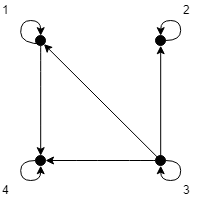
\includegraphics[scale=0.5]{7a-digraph.png}\\
	\end{center}
	\item \mbox{}
	\begin{center}
		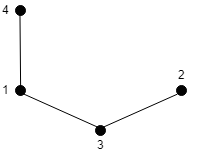
\includegraphics[scale=0.5]{7b-hasse-diagram.png}\\
	\end{center}
	\item Since a total order most have either $xRy$ or $yRx$ for every $x,y\in A$, and there are 2 of these occurrences in R, between 1 and 2, and 2 and 4.\\
	For each of these pairs there are 2 choices for our total ordering, one for each pair being ordered "after" the other for a total of $2^2=4$ total orders that contain the given partial order.
	\end{enumerate}
\item The number of equivalence relations on S with exactly 3 equivalence classes is the same as the number of ways to distribute 8 distinguishable elements between 3 indistinguishable boxes.\\
This number is $S(8,3)=966$
\end{enumerate}

\end{document}